\documentclass[11pt]{article}

\usepackage[margin=1in]{geometry}
\usepackage[T1]{fontenc}
\usepackage[utf8]{inputenc}
\usepackage{float}
\usepackage{lmodern}
\usepackage{amsmath}
\usepackage{booktabs}
\usepackage{graphicx}
\usepackage{hyperref}
\usepackage{url}
\usepackage{fancyhdr}
\setlength{\emergencystretch}{3em}

\title{CASCADE: A Software Framework and Synthetic Benchmark for Onboard Anomaly Triage}
\author{Emil Wes Lambert\\Delft University of Technology\\\texttt{e.w.lambert@student.tudelft.nl}\\\texttt{ORCID: 0000-0002-2459-9172}}
\date{Technical report, May 2026}

\begin{document}
\pagestyle{fancy}
\fancyhf{}
\fancyhead[L]{CASCADE technical report}
\fancyhead[R]{Lambert}
\fancyfoot[C]{\thepage}
\setlength{\headheight}{14pt}
\renewcommand{\headrulewidth}{0.3pt}
\maketitle

\begin{abstract}
CASCADE is an onboard anomaly-triage framework for downlink-bound Earth-observation missions: it screens each pass, updates a per-patch belief state, escalates uncertain scenes to multispectral/thermal fusion, and downlinks only compact alert products. A Crop Stress Composite (CSC) combines vegetation, thermal, and moisture-change indicators; a belief-gated policy selects among SKIP, screening, fusion, and priority-alert actions. In a 100-seed synthetic Monte Carlo benchmark, CASCADE reduces downlink by 99.05\% and energy use by 38.3\% relative to raw downlink while maintaining 100\% recall on injected anomaly events and a 0.6\% false-positive rate.

We evaluate CASCADE with the synthetic benchmark and reproducible MODIS real-scene replays. Real-scene replay is reported as a policy-stress and reproducibility test rather than a labelled drought benchmark: replay diagnostics show that maximum-pixel CSC thresholds can respond to sparse EVI/NDWI-driven field changes. The software therefore adds provenance-safe replay artifacts, source-bundle hashing, component attribution, spatial diagnostics, and a coherent-priority mode requiring p95 CSC, minimum alert fraction, and connected-component support.

CASCADE is released as an MIT-licensed framework for auditable onboard Earth-observation triage, where ``auditable'' means a deterministic decision trace (action timeline, thresholds, evidence state, and provenance hashes) sufficient to reproduce scheduling decisions from recorded inputs. Drought and crop-stress monitoring motivate the index choices; transfer to other hazards requires new indices, thresholds, and external validation.
\end{abstract}

\section{Introduction}

Earth-observation satellites can collect more imagery than they can downlink, process, or inspect immediately. Agricultural monitoring is an especially sharp case because early vegetation and moisture changes may be spatially local, while conventional workflows often downlink broad scenes for later ground processing \cite{mishra-singh-2010,nasa-challenge-brief}. CASCADE treats this as an onboard decision problem: each pass should decide whether to skip, screen, fuse additional channels, or downlink a compact priority product.

This technical report describes CASCADE as a reusable anomaly-triage and alert-downlink framework for crop-stress monitoring experiments. The strongest validated result is the controlled synthetic benchmark, where anomaly labels are known by construction. The real MODIS replay is intentionally narrower: it demonstrates replay infrastructure, provenance-safe artifacts, policy behavior, and failure modes of max-pixel alerting. It should not be read as completed drought-label validation.

This report makes four contributions:
\begin{enumerate}
\item a belief-gated onboard triage policy for crop-stress screening under resource constraints (Section~2);
\item a CSC fusion score combining vegetation, thermal, and moisture-change indicators (Section~2);
\item a synthetic benchmark with labelled injected anomalies, ablations, and sensitivity diagnostics (Section~3); and
\item a reproducible MODIS replay workflow with provenance-safe artifacts, component attribution, and coherent-priority diagnostics (Section~4).
\end{enumerate}

\section{Framework}

CASCADE combines a Crop Stress Composite with a lightweight belief gate. For patch $i$, the CSC combines vegetation loss, land-surface-temperature rise, and moisture loss:
\begin{equation}
\mathrm{CSC}_i =
w_E\frac{[E_{0,i}-E_i]_+}{s_E\sigma_E}
+w_L\frac{[L_i-L_{0,i}]_+}{s_L\sigma_L}
+w_N\frac{[N_{0,i}-N_i]_+}{s_N\sigma_N},
\label{eq:csc}
\end{equation}
clipped to $[0,1]$, where $[x]_+=\max(x,0)$. Here $\sigma_E$, $\sigma_L$, and $\sigma_N$ are fixed normalizers (EVI, LST [K], NDWI) that convert raw drops/rises to standardized anomaly magnitudes, and $s_E$, $s_L$, and $s_N$ are saturation constants that set the anomaly level at which each channel alone would reach a clipped value of $1.0$. The default weights are $0.578$, $0.246$, and $0.176$ for EVI, LST, and NDWI respectively.
In the reference implementation, each channel term is clamped to $[0,1]$ before weighting, and the weighted sum is then clipped again to $[0,1]$.

\begin{table}[H]
\centering
\caption{Default policy, CSC, and benchmark parameters (code: \texttt{src/cascade/core.py}).}
\label{tab:default-params}
\begin{tabular}{lll}
\toprule
Symbol / name & Default & Meaning \\
\midrule
$\sigma_E$ & 0.042 & EVI normalizer (approx. per-pass EVI noise scale) \\
$\sigma_L$ & 1.20 & LST normalizer in K (approx. per-pass LST noise scale) \\
$\sigma_N$ & 0.05 & NDWI normalizer (approx. per-pass NDWI noise scale) \\
$s_E$ & 7.0 & EVI saturation constant (units of $\sigma_E$-scaled drop) \\
$s_L$ & 4.956 & LST saturation constant (units of $\sigma_L$-scaled rise) \\
$s_N$ & 6.0 & NDWI saturation constant (units of $\sigma_N$-scaled drop) \\
$\tau_\mathrm{CSC}$ & 0.615 & CSC priority-alert operating threshold \\
$\tau_E$ & 0.18 & Stage-1 positive-evidence threshold in $\sigma_E$ units \\
$\tau_N$ & 0.12 & Stage-1 positive-evidence threshold in $\sigma_N$ units \\
$\Delta\alpha,\Delta\beta$ & 1 per screening & Beta pseudo-count updates (positive/negative) \\
$\alpha+\beta$ cap & 8 & Posterior evidence cap via rescaling \\
battery $b_\mathrm{crit}$ & 0.15 & SOC below which the policy returns SKIP \\
battery $b_\mathrm{cons}$ & 0.35 & SOC below which the policy returns MOD13 screening \\
$p_\mathrm{tail}$ gate & 0.70 & Tail-probability gate for escalation to fusion \\
$\mu$ gate & 0.55 & Posterior-mean gate for priority evidence \\
$n_\mathrm{evidence}$ & 2 & Minimum evidence pseudo-count for priority export \\
$n_\mathrm{explore}$ & 12 passes & Forced-FUSE cadence on stale posterior evidence \\
Alert packet & 1.8 MB & Per-tile alert-product size in benchmark \\
Priority overhead & 1.4 MB & Per-pass FUSE\_PRIORITY bundle header (compressed) \\
\bottomrule
\end{tabular}
\end{table}

\begin{table}[H]
\centering
\caption{Simplified energy and downlink model used in the benchmark. Per-pass energy is modeled as a fixed 30\,s active observation window per pass at constant action power (i.e., the action's payload + sensor + comms power drawn for 30\,s of effective acquisition/processing/downlink time per orbital pass; Table entries are derived from the hosted-payload component powers in \texttt{src/cascade/core.py}). Downlink volumes use the synthetic benchmark packet sizes (Table~\ref{tab:default-params}). For FUSE\_PRIORITY, the 1.4\,MB base term is a per-pass priority-bundle header (compressed indices, geotag, posterior summary, and provenance hashes) that is sent once per priority pass independent of alert count; the 1.8\,MB term is added once per promoted alert tile. With Full CASCADE the per-priority-pass average is roughly $1$ tile, yielding $\approx 3.2$\,MB per priority pass.}
\label{tab:energy-model}
\begin{tabular}{lrrr}
\toprule
Action & Power (W) & Energy / pass (Wh) & Baseline downlink volume \\
\midrule
SKIP & 0.3 & 0.0025 & 0 \\
MOD13 screening & 5.5 & 0.0458 & 0.7 MB \\
FUSE & 7.6 & 0.0633 & 2.8 MB \\
FUSE\_PRIORITY & 9.6 & 0.0800 & 1.4 MB + (alert tiles)$\times$1.8 MB \\
\bottomrule
\end{tabular}
\end{table}

The CSC weights, saturation constants, and $\tau_\mathrm{CSC}=0.615$ operating threshold are selected by the repository's calibration sweep over disjoint synthetic train, validation, and test seed ranges: seeds 0--59 for search, 60--79 for validation ranking, and 80--99 for promotion checks. The coherent-priority spatial gate introduced below is a post-hoc diagnostic mode for replay analysis rather than a calibrated drought classifier.

Each patch keeps a bounded Beta posterior initialized at $\alpha_i=\beta_i=1$. Stage-1 screening increments positive evidence by $\Delta\alpha=1$ when standardized EVI or NDWI anomaly magnitudes exceed $\tau_E$ or $\tau_N$ (Table~\ref{tab:default-params}), and otherwise increments negative evidence by $\Delta\beta=1$. Evidence is bounded by capping $\alpha_i+\beta_i$ at 8 via rescaling while preserving the posterior mean. The policy then selects one of four actions: SKIP, MOD13 screening, FUSE, or FUSE\_PRIORITY. The tail probability $p_\mathrm{tail}=\max_i q_i$ with $q_i=\Pr(p_i>0.5\mid \mathrm{Beta}(\alpha_i,\beta_i))$ is a per-pass field-level summary: \emph{any single} patch with $q_i>\tau_\mathrm{tail}$ triggers field-wide escalation from MOD13 to FUSE on that pass, regardless of how many other patches remain quiet. To prevent indefinite suppression of FUSE under cold posteriors, the policy also forces FUSE every $n_\mathrm{explore}=12$ passes since the last fusion. FUSE\_PRIORITY additionally requires a downlink window, fused CSC above $\tau_\mathrm{CSC}$, and a belief-informed stress gate (posterior mean/tail plus minimum evidence). A downlink window in the benchmark is a duty-cycled contact opportunity (15\% of orbit nominal, widened slightly to 0.15--0.45 orbital phase so that belief-scheduled fusion occasionally overlaps availability). In the benchmark, the belief gate is best interpreted as a resource-allocation mechanism: the no-belief ablation retains the same synthetic recall and slightly lower false-positive rate, but requires substantially higher seasonal-average compute and downlink. This belief-driven triage complements earlier spacecraft autonomy and dynamic-targeting systems by focusing on when accumulated patch-level evidence justifies scarce onboard compute and downlink, rather than only replanning target acquisition \cite{aspen-spaceops,eo1-autonomy,dynamic-targeting}.

\begin{figure}[H]
\centering
\caption{Algorithm 1: CASCADE per-pass decision rule (deterministic default, pseudocode).}
\label{alg:cascade}
\begin{minipage}{0.98\linewidth}
\begin{verbatim}
Inputs per pass:
  battery SOC b in [0,1]
  downlink window flag d in {0,1}
  last CSC map C
  posterior per patch (alpha, beta)
  steps since last fusion k

Compute standardized anomalies:
  a_E = max(0, (E0 - E) / sigma_E)
  a_N = max(0, (N0 - N) / sigma_N)   (or 0 if NDWI unavailable)

If b < b_crit: return SKIP
If b < b_cons: return MOD13

If Stage-1 screening due and not clouded:
  If (a_E >= tau_E) or (a_N >= tau_N): alpha += 1 else beta += 1
  Cap evidence by rescaling so alpha + beta <= 8
    while preserving alpha/(alpha+beta)

For each patch i, set q_i = P(p_i > 0.5) for p_i ~ Beta(alpha_i, beta_i)
Set p_tail = max_i q_i  (any patch with q_i > tau_tail
                         triggers field-wide escalation)

If (p_tail > tau_tail) or (k >= n_explore): action = FUSE else action = MOD13

If action == FUSE:
  Fuse and compute CSC map C' using Eq. (1)
  If d==1 and max(C') >= tau_CSC and belief-priority-gate passes:
    return FUSE_PRIORITY

return action
\end{verbatim}
\end{minipage}
\end{figure}

CASCADE is intended as a hosted-payload autonomy layer rather than a standalone spacecraft. The following hardware mapping is design intent rather than flight-demonstrated performance: radiometric preprocessing and pixel-level indices on a radiation-tolerant FPGA-class device, policy logic on a LEON4FT-class processor, degradation from fusion to Stage-1 screening under low battery state (Table~\ref{tab:default-params}), and export of compact geotagged alert packets rather than closed-loop agronomic prescriptions \cite{xilinx-wp523,ccsds-122}. The software model therefore emphasizes traceable rules, explicit resource gates, and reproducible alert products instead of an opaque learned controller.

\begin{figure}[H]
\centering
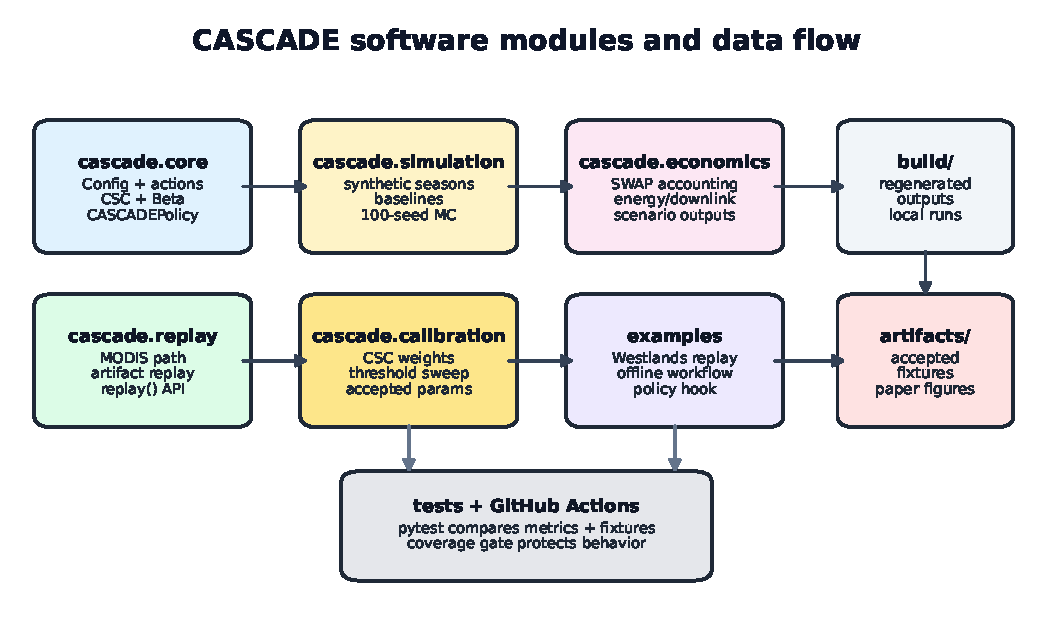
\includegraphics[width=\linewidth]{../figures/Figure_1_architecture.pdf}
\caption{CASCADE software and policy architecture. The onboard policy uses battery state, cadence, and posterior stress evidence to decide whether a pass remains at screening or escalates to fusion and alert downlink.}
\label{fig:architecture}
\end{figure}

\section{Synthetic Benchmark}

The synthetic benchmark runs 100 seeded seasons over 500 field patches and 120 orbital passes per seed. Here a ``patch'' is an independent per-pass time series representing a field-sized target unit in the benchmark (not a single satellite pixel); patches are treated as conditionally independent so that scheduler behavior can be measured at scale. Injected anomaly events provide labels for recall and false-positive accounting, while benign confounders and cloud-obscured passes stress the policy. This benchmark remains the quantitative validation anchor because the labels are controlled.

\subsection{Synthetic Anomaly Model}

Each seed draws per-patch baseline EVI, LST, and NDWI values from broad agricultural ranges and holds them fixed as the baseline terms $(E_{0,i},L_{0,i},N_{0,i})$ for that synthetic season (uniform draws: $E_{0,i}\!\sim\!U(0.42,0.70)$, $L_{0,i}\!\sim\!U(294.5,305.5)$\,K, $N_{0,i}\!\sim\!U(0.08,0.32)$). Seasonal sinusoidal variation and Gaussian sensor-like noise are then added around these baselines to produce per-pass observations. Twenty-one labelled stress patches per seed receive progressive anomalies with randomized onset between passes 18 and 72. The injected stress depresses EVI by up to 0.22, raises LST by up to 4.0 K, and mildly depresses NDWI by up to 0.03 over a 22-pass ramp; truth labels begin once severity exceeds 0.10. Nine benign confounder patches per seed receive shorter irrigation- or management-like events with randomized onset between passes 12 and 90 and duration of 4--10 passes; these depress EVI by up to 0.18, raise LST by up to 3.4 K, and impose stronger NDWI decline of up to 0.18, but are not labelled anomalies. Independently, each pass has a 0.30 cloud-obscuration probability that blocks useful sensing for that pass. These synthetic labels test scheduler behavior under a known generator; they are not a substitute for agronomic ground truth.

\subsection{Policies and Ablations}

We compare five policies in the benchmark implementation (\texttt{src/cascade/simulation.py}). RAW\_DUMP (figure label ``Raw downlink'') downlinks everything. FIXED\_ONBOARD (figure label ``Fixed onboard'') always runs fusion each pass and exports priority packets when a contact window exists and CSC exceeds $\tau_\mathrm{CSC}$. Full CASCADE (figure label ``Full CASCADE'') uses the belief-gated policy (Algorithm~1) to decide when to escalate to fusion and when to export priority tiles. The ABLATE\_NO\_BELIEF variant (figure label ``No belief'') removes the stored Beta posterior by triggering fusion only on the current-pass EVI/NDWI anomalies, isolating the value of temporal evidence accumulation. The EVI\_ONLY\_THRESHOLD baseline (figure label ``EVI only'') is an index-only alert filter that screens every pass and exports tiles only when standardized EVI anomaly exceeds a tuned threshold; it matches CASCADE's downlink order of magnitude but serves as a false-alert burden baseline.

Detection counting in the synthetic benchmark is per-pass and per-patch: on a given pass $t$, a patch $i$ contributes a true-positive (TP) tile if both $\mathrm{CSC}_i\geq\tau_\mathrm{CSC}$ and the injected truth label for $i$ is active at $t$; a false-positive (FP) tile if $\mathrm{CSC}_i\geq\tau_\mathrm{CSC}$ but the truth label is inactive. The reported false-positive rate is the seed-aggregated $\mathrm{FP}/(\mathrm{TP}+\mathrm{FP})$ over all detected per-pass tiles. The reported \emph{recall} is detector-level science retention: the fraction of injected stress patches in a seed for which at least one TP tile occurred at any pass during the simulation, averaged over seeds. This is a stricter metric than ``ever exceeded threshold somewhere in the field'' because the detector still has to fire on the right patch, but is looser than the priority-export latency in Figure~\ref{fig:detection-latency}, which counts only patches that triggered an actual FUSE\_PRIORITY downlink within a contact window.

Full CASCADE reduces downlink by 99.05\% relative to raw downlink and 77.6\% relative to a fixed onboard baseline. It reduces energy use by 38.3\% relative to raw downlink and 25.4\% relative to fixed onboard processing, while preserving 100.0\% \emph{detector-level} recall over the injected synthetic anomaly set at a 0.6\% per-tile false-positive rate. Across seeds, the 95\% confidence interval is 99.03--99.07\% for downlink reduction, 38.20--38.38\% for energy saving, 100.0--100.0\% for detector-level recall, and 0.43--0.78\% for the false-positive rate. The repository also includes a CSC-threshold ROC sweep over $\tau_\mathrm{CSC}$ with the 0.615 operating point recorded in the benchmark artifacts. Note that downlink volume alone does not separate Full CASCADE from the EVI-only ablation; the operationally decisive axis is the false-positive rate, where EVI-only (2.3\%) carries roughly four times the false-alert burden of Full CASCADE (0.6\%) at comparable downlink and recall.

The 100\% detector-level recall and the 15.4\% never-promoted fraction reported in Figure~\ref{fig:detection-latency} are not in tension: they measure different things. \emph{Detector-level recall} counts injected stress patches that the detector fires on at least once during a simulated season. \emph{Priority-export reach} counts injected stress patches that additionally pass the FUSE\_PRIORITY belief gate during a contact window. The 323/2100 (15.4\%) never-promoted patches were detected by the CSC at fusion time (so they contribute to the 100\% recall), but their fusion passes never coincided with a downlink window in which the belief-priority gate also fired, so they did not produce an explicit priority-alert tile. This is a deliberate property of the duty-cycled contact model and is the operational reason Figure~\ref{fig:detection-latency} reports priority-alert latency rather than threshold-exceedance latency.

To address the NDWI contribution question, we run an NDWI-removal ablation that disables NDWI in both Stage-1 belief updates and the CSC fusion computation. On this synthetic generator, recall remains 100\% but the false-positive rate increases from 0.6\% (95\% CI 0.43--0.78) to 1.2\% (95\% CI 0.97--1.43), indicating that NDWI helps suppress benign confounders that primarily express moisture-change signals. This does not establish that NDWI is essential for real drought detection; it only supports the claim that the three-channel CSC is not a cosmetic addition in the benchmark family.

\begin{figure}[H]
\centering
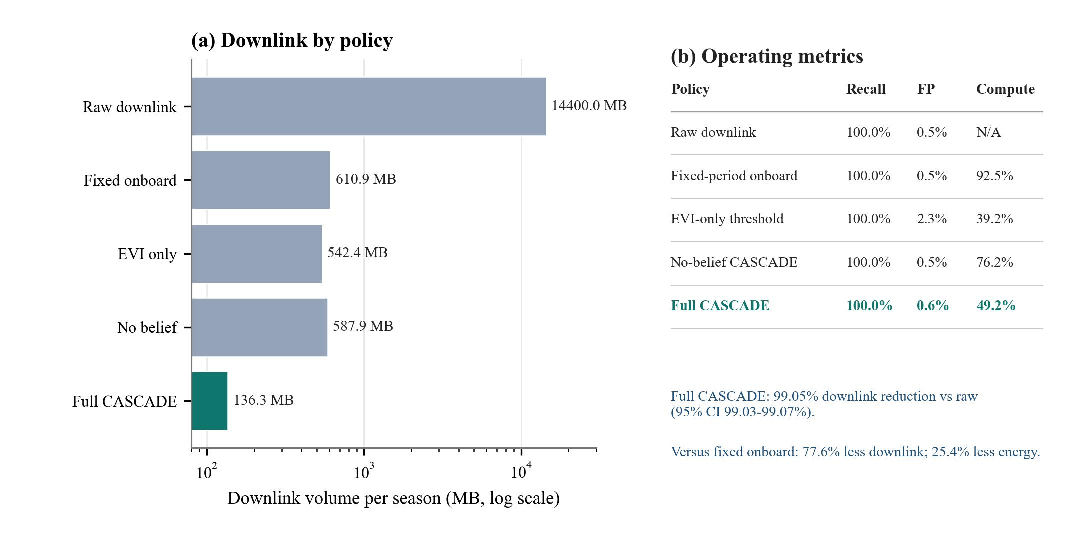
\includegraphics[width=\linewidth]{../figures/Figure_2_baseline_comparison.pdf}
\caption{Synthetic 100-seed Monte Carlo benchmark. Full CASCADE preserves recall on injected anomaly events while sharply reducing downlink and energy demand. The ``Compute'' column in panel (b) is the seasonal-average compute utilisation as a fraction of LEON4FT-class peak DMIPS, weighted by the per-action mix over the simulation (i.e., seed-averaged \texttt{seasonal\_average\_compute\_utilisation\_pct} in \texttt{src/cascade/simulation.py}); ``N/A'' for raw downlink reflects that no onboard compute is incurred. Policy labels in panel (b) map to \texttt{src/cascade/simulation.py} as: Raw downlink~$=$~RAW\_DUMP, Fixed onboard~$=$~FIXED\_ONBOARD, EVI only~$=$~EVI\_ONLY\_THRESHOLD, No belief~$=$~ABLATE\_NO\_BELIEF, Full CASCADE~$=$~CASCADE\_MDP.}
\label{fig:benchmark}
\end{figure}

\begin{figure}[H]
\centering
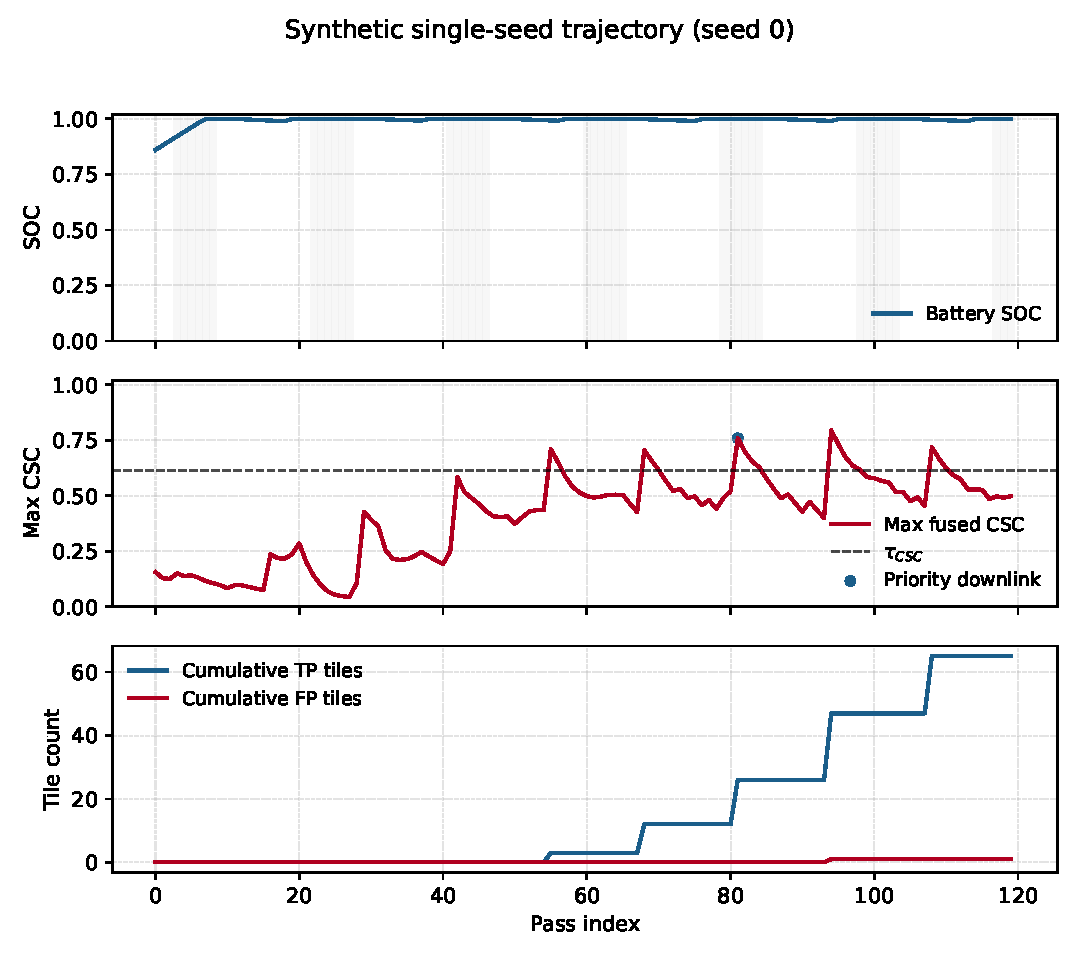
\includegraphics[width=\linewidth]{../figures/Figure_4_synthetic_trajectory.pdf}
\caption{Single-seed synthetic trajectory (seed 0). Battery SOC evolves under the simplified energy model (Table~\ref{tab:energy-model}); max CSC crosses $\tau_\mathrm{CSC}$ intermittently, and priority downlink occurs only when a contact window and belief gate coincide.}
\label{fig:trajectory}
\end{figure}

\begin{figure}[H]
\centering
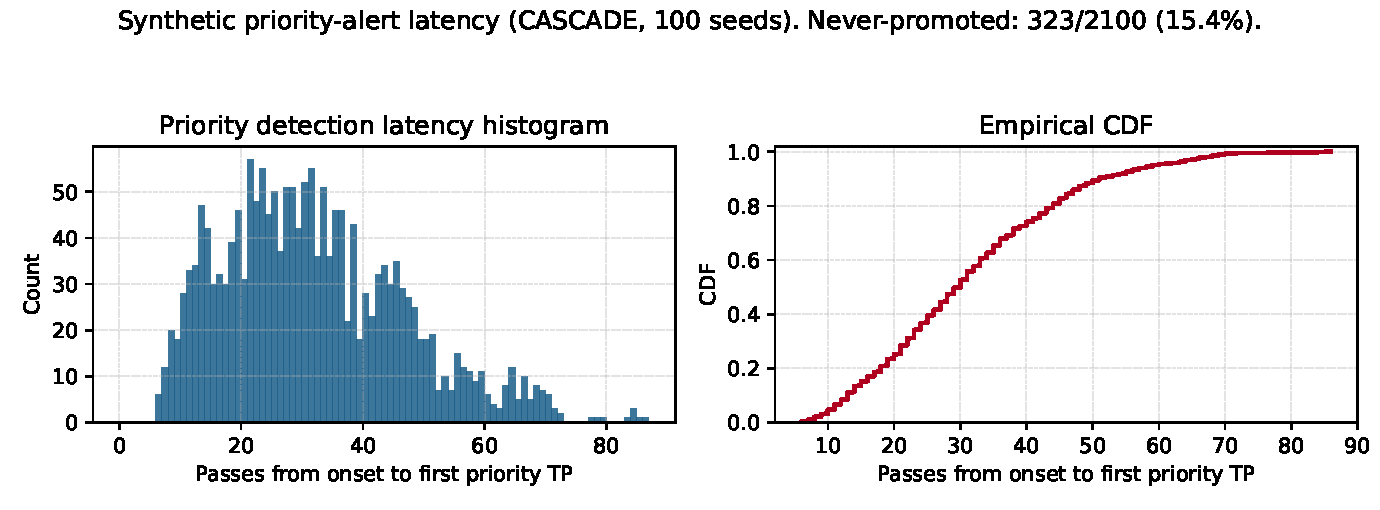
\includegraphics[width=\linewidth]{../figures/Figure_5_detection_latency.pdf}
\caption{Synthetic detection-timing diagnostic: distribution of passes from injected-anomaly onset to the first priority downlink that detects that patch. This measures \emph{priority export} latency (not merely threshold exceedance), and is therefore sensitive to downlink-window duty cycle and belief gating.}
\label{fig:detection-latency}
\end{figure}

\begin{figure}[H]
\centering
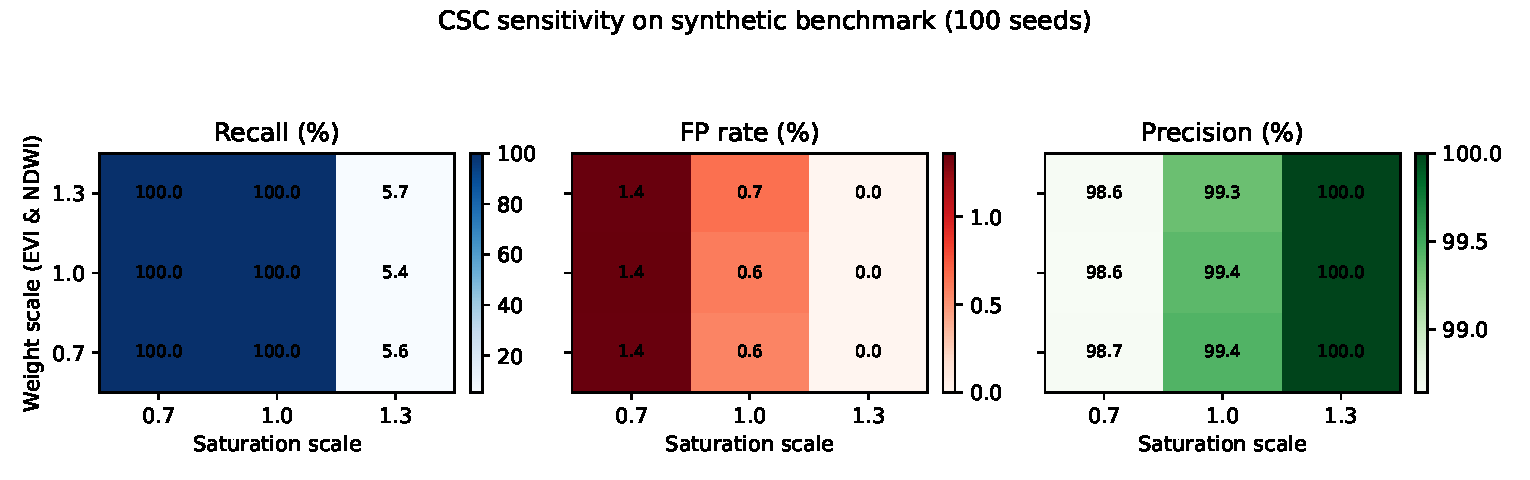
\includegraphics[width=\linewidth]{../figures/Figure_6_csc_sensitivity.pdf}
\caption{Sensitivity of benchmark recall and false-positive rate to multiplicative perturbations of CSC weights (EVI and NDWI scaled together) and saturation constants. This diagnostic addresses how much the headline metrics depend on a narrow calibration point within the synthetic generator family.}
\label{fig:csc-sensitivity}
\end{figure}

The CSC sensitivity diagnostic in Figure~\ref{fig:csc-sensitivity} shows a sharp, asymmetric failure mode at the high-saturation edge of the sweep: when saturation constants are scaled by $1.3$, the per-channel anomaly signal saturates so far above the operating threshold that detector-level recall collapses from $\geq 99.95\%$ to roughly $5.4$--$5.7\%$, while the false-positive rate drops to $0.0\%$ because almost no tile is ever flagged. Across the same grid, perturbing the EVI/NDWI weight scale by $\pm 30\%$ has no measurable effect on recall and only $\approx 0.05$ percentage points on the false-positive rate (Figure~\ref{fig:csc-sensitivity}). This cliff-edge behaviour means the calibration is robust to weight-balance error within roughly $\pm 30\%$ but only modestly robust to a global rescaling of the saturation constants: an underestimate of the true per-channel anomaly amplitude in the synthetic generator family would push the operating point past the saturation knee and silently zero recall. The implication is that real-data deployment must re-estimate saturation constants on representative ground truth before reusing $\tau_\mathrm{CSC}$, rather than treating the synthetic-calibrated saturation values as portable defaults.

\section{Reproducible MODIS Replay and Policy-Stress Diagnostics}

The MODIS replay path aligns AppEEARS V061 MOD13A1, MOD11A1, and MOD09A1 products over the Westlands/Firebaugh AOI, computes rolling-baseline CSC values, and replays the same policy over historical windows \cite{mod13a1,mod11a1,mod09a1,mod09-guide}. The rolling baseline used in the current replay implementation is a per-pixel median over the prior three valid replay windows (a warmup of three valid windows is required before alerting). LST and NDWI windows are computed as 16-day medians aligned to the 16-day MOD13A1 cadence. The current replay artifacts record AOI name, bounding box, date range, code commit, AppEEARS task ID, input layers, deterministic source-bundle hash, creation time, and whether a CSC stack is present.

The stricter coherent-priority mode makes the spatial evidence requirement explicit. Let $f_\mathrm{alert}$ be the fraction of finite replay pixels with $\mathrm{CSC}\geq\tau_\mathrm{CSC}$ and let $C_\mathrm{max}$ be the largest connected alert component in pixels. A fused scene is eligible for coherent FUSE\_PRIORITY only if the existing downlink-window, posterior, evidence, and max-CSC pre-gates pass and
\[
\mathrm{CSC}_{p95} \geq 0.615,\qquad
f_\mathrm{alert} \geq 0.05,\qquad
C_\mathrm{max} \geq 4.
\]
This gate is designed to suppress single-pixel or two-pixel CSC spikes while keeping the legacy max-pixel rule available for backward-compatible policy stress tests. The three thresholds were chosen to enforce three distinct evidence requirements rather than to pass a single tuned target: $\mathrm{CSC}_{p95}\geq\tau_\mathrm{CSC}$ requires that at least the top $5\%$ of finite pixels (and not just the maximum pixel) cross the same operating threshold used in the synthetic benchmark; $f_\mathrm{alert}\geq 0.05$ requires that the alert area exceed sensor-noise-level isolated triggers under the AOI's pixel count; and $C_\mathrm{max}\geq 4$ requires connected spatial support, which is the smallest connected component that is unlikely under independent per-pixel noise on the AOI grid. We deliberately do \emph{not} re-tune these to maximize replay alerts, since the replay does not have ground-truth drought labels; the gate is a spatial-coherence diagnostic, not a calibrated drought classifier.

The corrected current-AOI replay does not support the earlier drought-vs-quiet separation narrative. An earlier internal replay comparison used a stale Westlands 2024 artifact generated from an older AOI definition; regenerating both seasons with the current Westlands/Firebaugh AOI removes the reported quiet-year separation. Legacy max-CSC replay reaches peak CSC 0.869 in 2014 and 0.865 in 2024, with priority alerts in both seasons. The 2014 alert fraction is roughly twice the 2024 alert fraction, but both remain below the coherent-priority spatial-support threshold. The updated coherent-priority mode therefore suppresses both seasons because the alert fields are spatially sparse under the p95, alert-fraction, and connected-component gate. This is useful evidence about the software and policy, but it is not a drought-label validation result.

\begin{table}[H]
\centering
\caption{Westlands current-AOI replay diagnostics. Legacy max-CSC mode promotes sparse alert pixels in both years; coherent-priority mode suppresses both because p95 CSC, alert fraction, and connected-component support are insufficient for spatially coherent priority evidence.}
\label{tab:replay-diagnostics}
\resizebox{\linewidth}{!}{%
\begin{tabular}{lrrrrrr}
\toprule
Case & Legacy alerts & Coherent alerts & Max CSC & p95 CSC & Alert fraction & $C_\mathrm{max}$ \\
\midrule
Westlands 2014 & 6 & 0 & 0.869 & 0.556 & 0.042 & 3 \\
Westlands 2024 & 5 & 0 & 0.865 & 0.243 & 0.021 & 2 \\
\bottomrule
\end{tabular}
}
\end{table}

\begin{figure}[htbp]
\centering
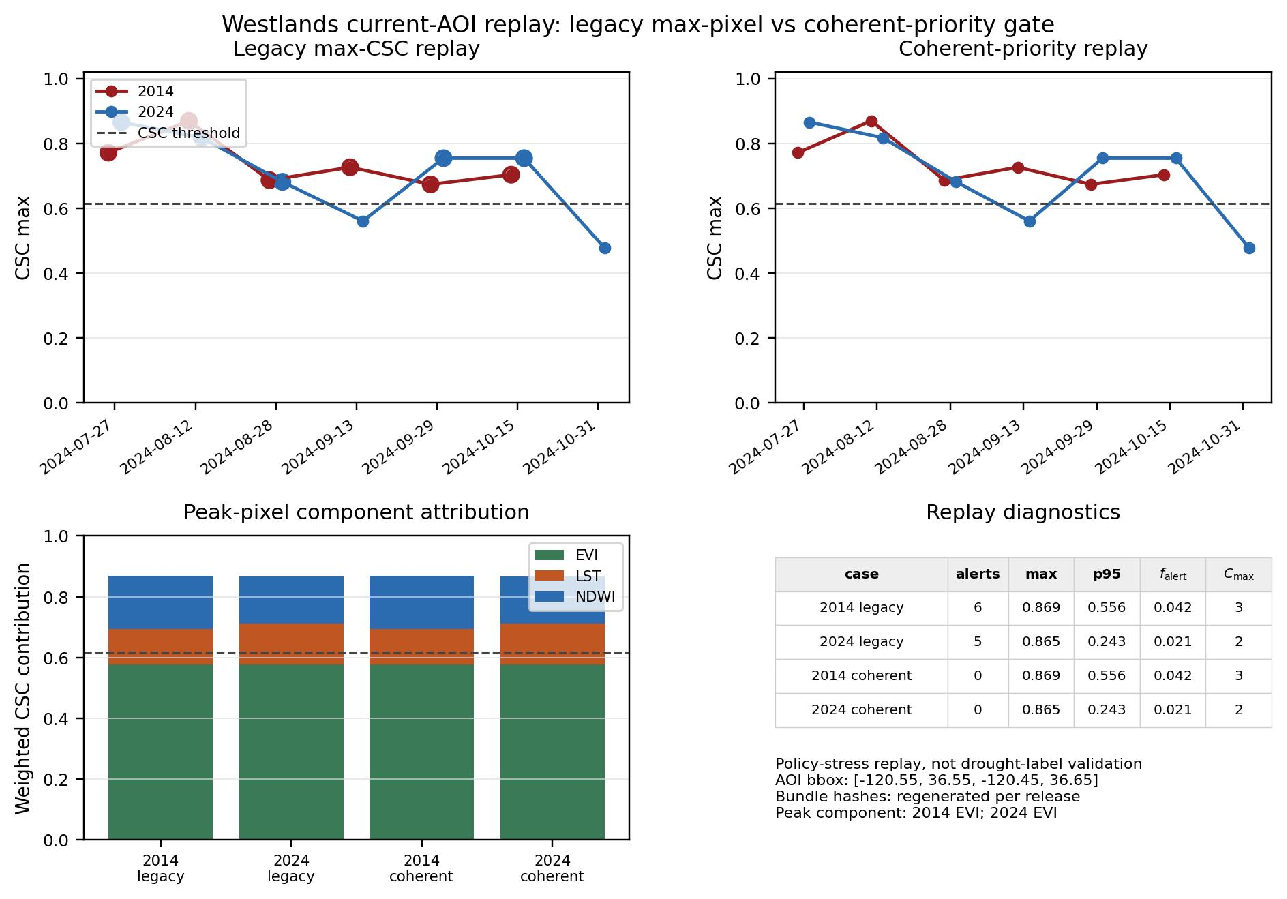
\includegraphics[width=\linewidth]{../figures/Figure_3_replay_modes.pdf}
\caption{Legacy max-CSC versus coherent-priority replay. Legacy max-CSC replay is sensitive to sparse field-level EVI/NDWI changes; coherent-priority mode suppresses these sparse triggers by requiring p95 CSC, minimum alert fraction, and connected-component support.}
\label{fig:replay-modes}
\end{figure}

\section{Reproducibility}

The repository contains Python package code, accepted JSON fixtures, replay artifacts, CSC stacks, and paper-generation scripts. It targets Python $\geq 3.10$ ($<3.13$); runtime dependencies (\texttt{numpy}, \texttt{pandas}, \texttt{matplotlib}, \texttt{rasterio}, \texttt{requests}, \texttt{tqdm}) and the optional \texttt{pytest} test extras are pinned in \texttt{pyproject.toml}. The fast path is:
\begin{verbatim}
python -m pytest -q
python -m cascade.simulate
python -m cascade.replay --year 2014 --priority-mode legacy_max
python -m cascade.replay --year 2024 \
  --priority-mode coherent_priority --no-prefer-artifacts
\end{verbatim}
The lower-level AppEEARS workflow can regenerate live MODIS replay outputs when credentials and dependencies are available; otherwise, tracked artifacts provide offline reproducibility for review.

\section{Limitations}

CASCADE is pre-flight research software. The synthetic benchmark validates scheduler behavior under known injected anomalies, not agronomic causality. The real-scene MODIS replay demonstrates policy execution, provenance, and spatial diagnostics, but external drought labels and multi-region ground truth remain future work.

The current anomaly generator is intentionally simple: progressive EVI/LST/NDWI changes, short benign confounders, and pass-level cloud masks. Its 100.0\% recall should therefore be read as full recall over this controlled injected anomaly set, not as evidence that crop stress is generally easy to detect. The CSC weights and legacy threshold are calibrated within that synthetic family, and the coherent-priority gate is only a replay diagnostic until evaluated across independent labelled regions. Because calibration is performed exclusively on synthetic seeds (Section~2), the same weights, saturations, and $\tau_\mathrm{CSC}$ values are not guaranteed to transfer to real MODIS data: distribution shift in EVI/LST/NDWI noise scale, baseline phenology, irrigation, and cloud-correlated coverage can all move the operating point off the calibrated knee shown in Figure~\ref{fig:csc-sensitivity}, and the replay therefore reports only policy behaviour, provenance, and spatial diagnostics rather than a drought-validation result.

The MODIS replay uses MOD13A1 EVI at 500\,m; ``field-level'' framing can therefore be misleading for sub-pixel parcels or mixed crop mosaics, and sparse CSC spikes may reflect management or phenology rather than drought. The current rolling-baseline CSC is sensitive to phenology, harvest, irrigation, and field-management changes; users should not interpret max-pixel CSC alone as a drought detector.

The synthetic generator is intentionally simple and therefore does not fully stress confounding: benign confounders differ in duration and NDWI magnitude from labelled stress events; cloud obscuration is i.i.d.\ per pass rather than spatially correlated; and the tight confidence intervals suggest limited inter-seed diversity within this generator family. The paper also does not include comparisons to external vegetation-anomaly baselines (e.g., VCI or z-score NDVI/EVI anomaly) or operational detection-latency analyses; these are future-work items for domain validation beyond the policy-scheduler focus of this report. Hardware, orbital, and SmallSat constraints beyond the duty-cycled contact and simplified energy model are likewise design constraints for future work rather than flight-demonstrated performance.

\section{Conclusion}

CASCADE demonstrates an auditable onboard triage framework for crop-stress anomaly screening under SmallSat resource constraints. Its primary quantitative result is synthetic: large downlink and energy savings with full recall over the controlled injected anomaly set. The benchmark supports the software claim that belief-gated fusion and alert downlink can reduce resource use while preserving injected-event recall under a known generator. It does not establish field-level agronomic causality or drought discrimination. The real-scene contribution is reproducibility infrastructure and policy-stress analysis: provenance-safe replay artifacts, source-bundle hashing, component attribution, spatial diagnostics, and a coherent-priority mode. The corrected Westlands replay is especially useful as a failure-mode example because it shows how max-pixel CSC can react strongly to sparse field changes in both comparison years. Drought-specific validation against external labels remains future work. The intended role of this report is therefore to publish a clean software and benchmark record, not to close the remote-sensing validation problem.

\section*{Data and Code Availability}

The MIT-licensed source code and accepted artifacts are available at \url{https://github.com/emillambert/CASCADE}; \texttt{LICENSE.txt} is the canonical repository license file. The companion software release is tagged \texttt{v1.1.0-arxiv}.

\section*{Conflict of Interest}

The author declares no competing interests.

\section*{Acknowledgements}

This work uses MODIS Terra/Aqua land products (MOD13A1, MOD11A1, MOD09A1) accessed through the NASA AppEEARS service operated by the Land Processes Distributed Active Archive Center (LP DAAC). The author thanks the AppEEARS and LP DAAC teams for maintaining the analysis-ready interface used by the replay pipeline, and the NASA SmallSat / Space-to-Soil challenge organizers whose framing motivated the original onboard-triage formulation. No external funding supported this technical report. The author also thanks the open-source maintainers of \texttt{numpy}, \texttt{matplotlib}, \texttt{pandas}, and \texttt{rasterio}, on which the framework depends.

\newpage
\bibliographystyle{unsrt}
\bibliography{../references}

\end{document}
